\begin{figure}[t]
        \centering
	\begin{subfigure}[b]{0.54\textwidth}
	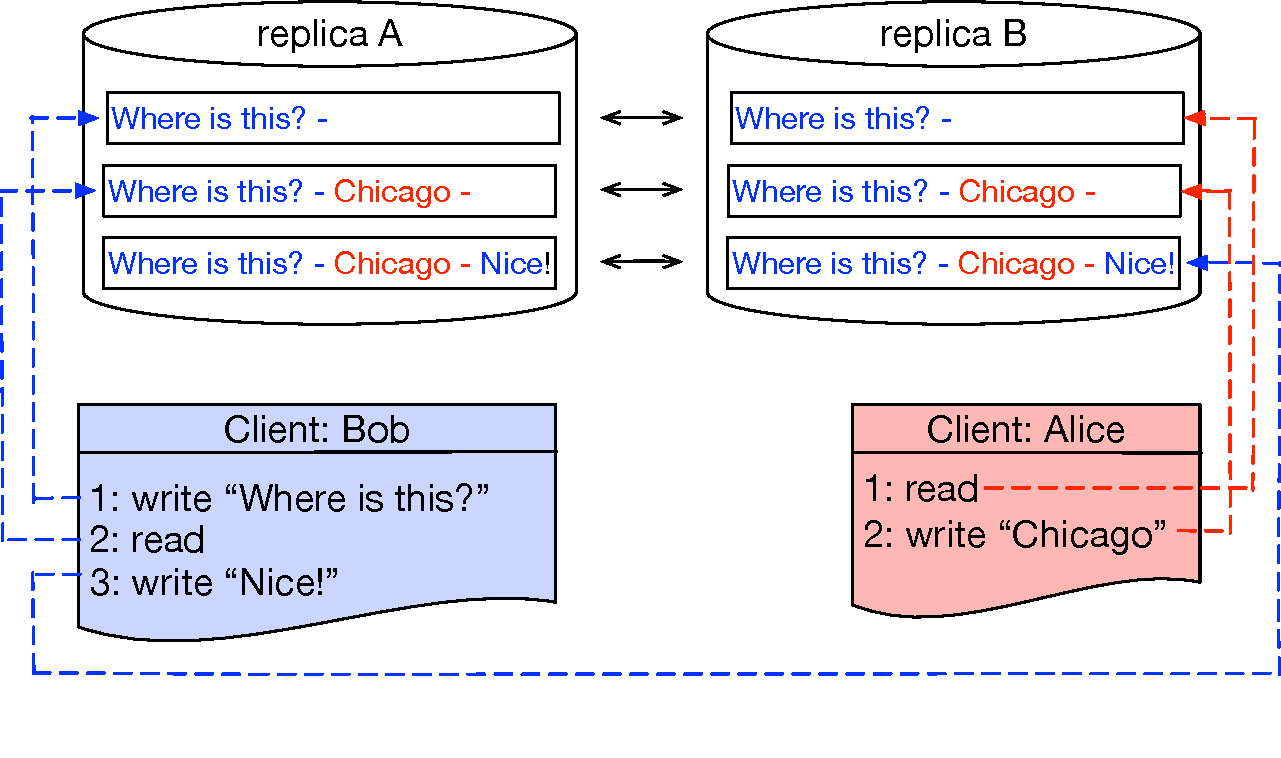
\includegraphics[scale=0.36]{Figures/comment_application.pdf}
	\label{comment_example}
	\end{subfigure} 
	\begin{subfigure}[b]{0.45\textwidth}
	\begin{lstlisting}
	data Effect = Eff String 
	type State = String 

	read :: State -> (String, Maybe Effect)
	read s = (s,Nothing)

	write :: String -> ((), Maybe Effect)
	write comment = ((), Just (Eff comment))

	apply :: State -> Effect -> State 
	apply s eff = let Eff comment = eff
		        	  in s ++ " - " ++ comment
	\end{lstlisting}
	\label{subfig:comment_code}
	\end{subfigure}
\\ \hrulefill
\caption{A distributed comment section applicataion, serving two clients
(left) and its implementation in \tool (right)}
\label{fig:comment_app}
\end{figure}


